\chapter{协变电动力学}\label{ch:b3:covariant-electromagnetism}

一根铜导线中通有十安培电流。其中电子的漂移速率
仅为每秒十分之一毫米，比蜗牛还慢，
而导线在极高的精度下仍呈电中性。然而，
与一个电荷并排运动的另一电荷
仍会感受到可测量的拉力。若从该电荷自身所在的
参考系来看，“磁”的解释便消失了：电荷静止，
而静止的电荷不受任何磁力。在该参考系中，拉住它的是一个
\emph{电}场。它由相对论本身产生，因为长度收缩
使导线中两股电荷流失去平衡，失衡的程度为
$10^{24}$ 分之一。磁不过是从运动的座位上所见的电。
本章用前三章的语言改写本科二年级分册中的电磁学：
电荷与势用四维矢量表示，$\vect E$ 与 $\vect B$
合并于同一个反对称张量，麦克斯韦四个方程
合并为两行，且在每个惯性参考系中形式相同。
除了形式上的简洁，更重要的是物理应用：
场如何变换，为何快速运动电荷的场会压扁成一张饼，
以及相对论性电子的光为何像车头灯一样
向前扫射——这正是
今天用于 X 射线探测蛋白质与电池的同步辐射光源的原理。

\section{电荷与电流的四维矢量}

\begin{definition}[四维矢量]\label{def:b3:covariant-electromagnetism:fourvector}
\index{四维矢量}
称\emph{四维矢量}为四元组 $a^\mu = (a^0, \vect a)$，$\mu =
0, 1, 2, 3$，其分量在洛伦兹变换下的混合方式恰与 $(ct,
\vect r)$ 的分量一致：
\[
a'^0 = \gamma(a^0 - \beta a^1) , \qquad
a'^1 = \gamma(a^1 - \beta a^0) , \qquad
a'^{2,3} = a^{2,3}
\]
对速率为 $\beta c$、沿 $x$ 方向的洛伦兹变换而言，任意两个四维矢量给出
不变标量积 $a\cdot b = a^0b^0 - \vect a\cdot\vect b$，
在每个参考系中都是同一个数，这正是 $c^2t^2 - x^2$
与 $E^2 - p^2c^2$ 背后的规律。位置 $(ct, \vect r)$ 与四维动量
$(E/c, \vect p)$ 是我们已有的两个；电磁学现在又提供三个：
电流、势与波矢。
\end{definition}

\begin{proposition}[四维电流与电荷守恒]\label{prop:b3:covariant-electromagnetism:fourcurrent}
\index{四维电流}
电荷密度 $\rho$ 与电流密度 $\vect\jmath$
构成四维电流
\[
J^\mu = (\rho c,\ \vect\jmath\,) :
\]
一团固有电荷密度为 $\rho_0$、以 $\vect u$ 运动的电荷云，
具有 $J^\mu = \rho_0\gamma_u(c, \vect u)$——其密度增大为 $\gamma_u$ 倍，
原因是电荷云的体积收缩，而电荷本身
是不变量（一个决定性的实验事实：内层电子运动很快的原子
仍严格呈电中性）。电荷守恒是一条
不变的表述：
\[
\frac{\partial(\rho c)}{\partial(ct)} +
\operatorname{div}\vect\jmath = 0 ,
\]
即本科二年级分册中的连续性方程，如今清楚地表明
它对所有观测者都是同一条规律。
\end{proposition}

\begin{proof}[部分证明]
运动的电荷云：一个固有体积为 $V_0$ 的盒子内含电荷 $\rho_0
V_0$；在实验室中该盒子收缩为 $V_0/\gamma_u$，因此 $\rho =
\gamma_u\rho_0$，由电流密度的定义有 $\vect\jmath = \rho\vect u$。
$(\rho c, \vect\jmath)$ 能作为四维矢量变换，依据在于它等于
$\rho_0/c$ 乘以四维速度 $\gamma_u(c, \vect u)$，
而后者按构造本身就是四维矢量。
电荷不变性则是一个实验输入。
\end{proof}

\section{用一个张量表示两个场}

\begin{definition}[四维势与电磁场张量]\label{def:b3:covariant-electromagnetism:tensor}
\index{四维势}\index{电磁场张量}
本科二年级分册中的各个势组合为四维势
\[
A^\mu = \Big(\frac{V}{c},\ \vect A\Big) ,
\]
而可测量的场 $\vect E = -\vect\nabla V -
\partial_t\vect A$，$\vect B = \operatorname{\vect{curl}}\vect A$ 是
同一个反对称阵列的六个独立分量，即
\emph{电磁场张量}
\[
F^{\mu\nu} =
\begin{pmatrix}
0 & -E_x/c & -E_y/c & -E_z/c\\
E_x/c & 0 & -B_z & B_y\\
E_y/c & B_z & 0 & -B_x\\
E_z/c & -B_y & B_x & 0
\end{pmatrix} .
\]
$\vect E$ 与 $\vect B$ 并非两个场，而是同一对象的
六个面；观测者把哪一个面称为“电”，取决于
观测者自身的运动。
\end{definition}

\begin{theorem}[麦克斯韦方程组的协变形式]\label{thm:b3:covariant-electromagnetism:maxwell}
\index{麦克斯韦方程组!协变形式}
本科二年级分册中的四个麦克斯韦方程，是
两条与参考系无关的陈述的分量形式：有源的一对
（高斯定律与安培–麦克斯韦定律）为
\[
\sum_\mu \partial_\mu F^{\mu\nu} = \mu_0\,J^\nu ,
\]
而无源的一对（无磁单极子，法拉第定律）则是恒等式，
保证 $F$ 可由四维势导出。洛伦兹
力为 $\dd p^\mu/\dd\tau = qF^{\mu\nu}u_\nu$——力的定律，
磁力也包括在内，一行即可写出。由于方程的两边
在变换下完全相同，\emph{麦克斯韦理论无需修正
即可满足相对论的要求}：它是相对论的第一块
完成的成果，诞生于 1865 年。
\end{theorem}

\begin{proof}[部分证明]
展开 $\nu = 0$ 分量：$\sum_i\partial_i(E_i/c) =
\mu_0\rho c$，即 $\operatorname{div}\vect E = \rho/\varepsilon_0$
（利用 $c^2 = 1/\mu_0\varepsilon_0$）。$\nu = 1$ 分量
包含 $-\partial_t(E_x/c^2) + (\partial_yB_z - \partial_zB_y)
= \mu_0 j_x$，即安培–麦克斯韦方程的 $x$ 分量。其余
分量同理；无源的一对即
$A^\mu$ 的交叉二阶导数相等（
在\cref{exo:b3:covariant-electromagnetism:3}中验证）。$F^{\mu\nu}$
按（二指标）张量变换——每个指标都像四维矢量——
这一点在本阶段不加证明地承认；其推论即下一命题。
\end{proof}

\section{场如何变换}

\begin{proposition}[场的变换]\label{prop:b3:covariant-electromagnetism:transform}
\index{场的变换}
对速度为 $\vect v = v\,\vect e_x$ 的洛伦兹变换，分量
\emph{沿}运动方向的分量保持不变，横向分量相互混合，
\[
E'_x = E_x , \qquad
E'_y = \gamma(E_y - vB_z) , \qquad
E'_z = \gamma(E_z + vB_y) ,
\]
\[
B'_x = B_x , \qquad
B'_y = \gamma\Big(B_y + \frac{v}{c^2}E_z\Big) , \qquad
B'_z = \gamma\Big(B_z - \frac{v}{c^2}E_y\Big) .
\]
写成紧凑形式，横向于变换方向：$\vect E' = \gamma(\vect E +
\vect v\wedge\vect B)_\perp$ 与 $\vect B' = \gamma(\vect B - \vect
v\wedge\vect E/c^2)_\perp$。一个参考系中的纯 $\vect B$，在另一参考系中是 $\vect
E$ 与 $\vect B$ 的组合——场是同一种现象。
\end{proposition}
\admitted

\begin{example}[中性导线的磁性]\label{ex:b3:covariant-electromagnetism:wire}
一根中性导线通有电流：正离子晶格静止，电子
漂移。对旁边运动的试探电荷，变换到其参考系：两
股电荷流\emph{以不同方式}收缩（它们的速度不同），
导线获得净线电荷 $\lambda' =
-\gamma vI/c^2$，其径向电场以
恰好与实验室所称的 $q\vect v\wedge\vect B$ 一样的力拉动电荷。磁性
就是相对论的二阶项 $v u/c^2$ 在
$10^{28}$ 个元电荷每米协同作用时的表现：每种效应都极其微小，
但导线在更高精度上仍是中性的，
因此那微小的失衡便是全部的故事
（见\cref{pb:b3:covariant-electromagnetism:1}）。
\end{example}

\begin{omfigure}
\begin{tikzpicture}[font=\small, >=Stealth]
  % lab frame
  \begin{scope}
    \draw[thick, fill=omExo!10] (-0.2,0) rectangle (5.4,0.75);
    \foreach \x in {0.3,1.3,2.3,3.3,4.3} \node[omThm] at (\x,0.52) {$\oplus$};
    \foreach \x in {0.8,1.8,2.8,3.8,4.8} {\node[omDef] at (\x,0.22) {$\ominus$};
      \draw[->, omDef] (\x+0.16,0.22) -- (\x+0.42,0.22);}
    \fill[omProp] (2.6,-1.15) circle (2.6pt);
    \draw[->, omProp, thick] (2.75,-1.15) -- (3.55,-1.15);
    \node[anchor=west] at (3.65,-1.15) {$q$，速率 $v$};
    \draw[->, very thick] (2.6,-0.95) -- (2.6,-0.35);
    \node[anchor=west, font=\footnotesize] at (2.7,-0.62) {$q\vect v\wedge\vect B$};
    \node at (2.6,1.35) {实验室：导线中性，力为磁力};
  \end{scope}
  % charge frame
  \begin{scope}[xshift=7.8cm]
    \draw[thick, fill=omExo!10] (-0.2,0) rectangle (5.4,0.75);
    \foreach \x in {0.25,1.15,2.05,2.95,3.85,4.75} {\node[omThm] at (\x,0.52) {$\oplus$};
      \draw[->, omThm] (\x-0.14,0.72) -- (\x-0.4,0.72);}
    \foreach \x in {0.7,1.9,3.1,4.3} \node[omDef] at (\x,0.22) {$\ominus$};
    \fill[omProp] (2.6,-1.15) circle (2.6pt);
    \node[anchor=west] at (2.75,-1.35) {$q$，静止};
    \draw[->, very thick] (2.6,-0.95) -- (2.6,-0.35);
    \node[anchor=west, font=\footnotesize] at (2.7,-0.62) {$q\vect E'$};
    \node at (2.6,1.35) {电荷系：导线带电，力为电力};
  \end{scope}
\end{tikzpicture}

{\small 同一个力，两种算法。实验室：中性导线的电流
产生 $\vect B$，运动电荷受到 $q\vect v\wedge\vect B$。
电荷系：正离子晶格此时运动并收缩，
电子（在该系中较慢）分散开；导线带净电荷，其
$\vect E'$ 起拉动作用。同一实验，同一结果。}
\end{omfigure}

\begin{example}[快速电荷的扁平场]\label{ex:b3:covariant-electromagnetism:pancake}
将电荷的库仑场变换到其
$\gamma \gg 1$ 运动的参考系中：纵向场不变，而横向场
乘以 $\gamma$。原本球对称的场
压扁成张角 $\sim 1/\gamma$ 的盘状，围绕过电荷的
平面分布；在垂直于运动的方向上，伴有
磁环 $B' = vE'/c^2$。对静止观察者而言，
LHC 质子（$\gamma \approx 7000$）的经过是
亚皮秒量级、由近乎垂直的 $\vect E$ 与 $\vect B$ 构成的冲击：几乎
一束光脉冲——这正是快速束流与物质相互作用
方式与光子相仿的原因。
\end{example}

\begin{omfigure}
\begin{tikzpicture}[font=\small, >=Stealth]
  % static charge
  \begin{scope}
    \fill[omThm] (0,0) circle (2.6pt);
    \foreach \a in {0,30,...,330} \draw[->, omDef] (\a:0.25) -- (\a:1.75);
    \node at (0,-2.5) {静止：各向同性库仑场};
  \end{scope}
  % moving charge
  \begin{scope}[xshift=8.0cm]
    \fill[omThm] (0,0) circle (2.6pt);
    \draw[->, very thick] (0.3,-2.1) -- (1.5,-2.1) node[right] {$v \approx c$};
    \foreach \a/\l in {90/1.95, 75/1.5, 105/1.5, 60/0.85, 120/0.85,
                       270/1.95, 255/1.5, 285/1.5, 240/0.85, 300/0.85,
                       0/0.35, 180/0.35, 30/0.45, 150/0.45, 210/0.45, 330/0.45}
      \draw[->, omDef] (\a:0.25) -- (\a:\l);
    \node at (0,-2.5) {};
    \node at (0.3,-2.65) {};
    \node at (0,-2.9) {};
  \end{scope}
  \node at (8.0,-2.5) {运动：场压扁为 $\sim 1/\gamma$};
\end{tikzpicture}

{\small 点电荷的电场，静止与高速时：作洛伦兹推促使横向分量乘以 $\gamma$，
纵向分量保持不变，场被挤压成
一张
垂直于运动方向的圆盘。}
\end{omfigure}

\section{不变量、光与车灯效应}

\begin{proposition}[场的两个不变量]\label{prop:b3:covariant-electromagnetism:invariants}
\index{场的不变量}
由 $F^{\mu\nu}$ 可构造恰好两个独立的标量：
\[
E^2 - c^2B^2
\qquad\text{和}\qquad
\vect E\cdot\vect B ,
\]
在每个惯性参考系中取值相同。由此，若某处 $E > cB$，
（且 $\vect E\cdot\vect B = 0$），则存在某参考系在该处只看到纯电场；
若 $E < cB$，则存在某参考系只看到纯磁场；平面
光波满足 $E = cB$ 且 $\vect E\perp\vect B$，\emph{两个}
不变量都为零——它在每个参考系中都是光：任何洛伦兹推促都无法将其
变为静态场，只能使其红移。无法追上
一列光波；爱因斯坦少年时的疑问，
由两个不变量自行给出答案。
\end{proposition}

\begin{proof}[部分证明]
对标准洛伦兹推促检验不变性，直接代入
\cref{prop:b3:covariant-electromagnetism:transform}
（见\cref{exo:b3:covariant-electromagnetism:6}）；不存在第三个独立不变量这一点，在本阶段不加证明地承认。
对光波：$E = cB$ 与
正交性给出两者皆为零；若某参考系中有静态场，则需要
一个非零的不变量。
\end{proof}

\begin{proposition}[四维波矢、多普勒效应与光行差]\label{prop:b3:covariant-electromagnetism:wavevector}
\index{光行差}\index{车灯效应}
平面波的频率与方向构成零四维矢量
$k^\mu = (\omega/c, \vect k)$，$\|\vect k\| = \omega/c$。对其作变换，
立即得到在\cref{ch:b3:relativistic-kinematics}中的相对论多普勒公式，
以及方向的\emph{光行差}，
其形式为：
\[
\cos\theta' = \frac{\cos\theta - \beta}{1 - \beta\cos\theta} .
\]
反过来看，在静止参考系中各向同性辐射的源，
在实验室中把一半光射入前向锥 $\theta
\lesssim 1/\gamma$ 内，称为\emph{车灯效应}。
一个在储存环中以 $\gamma \sim 10^4$ 运动的电子，扫出
一束 $\qty{0.1}{mrad}$ 的 X 射线探照光，绕环扫过——即
充满蛋白质晶体学束线的同步辐射光。
\end{proposition}

\begin{proof}[部分证明]
相位 $\omega t - \vect k\cdot\vect r = k^\mu x_\mu$ 计数经过各事件的
波峰数（一个不变量），因此 $k^\mu$ 必须
按四维矢量变换。对 $(\omega/c, k\cos\theta,
k\sin\theta, 0)$ 作洛伦兹推促：时间分量给出多普勒效应，空间分量之比给出
光行差公式。令 $\theta' =
90^\circ$（源参考系中的侧向射线）：$\cos\theta =
\beta$，即 $\theta \approx 1/\gamma$（$\gamma \gg 1$）——
一半球面折入前向锥。
\end{proof}

\begin{omfigure}
\begin{tikzpicture}[font=\small, >=Stealth]
  % isotropic source
  \begin{scope}
    \fill[omThm] (0,0) circle (2.4pt);
    \foreach \a in {0,45,...,315} \draw[->, omExo] (\a:0.3) -- (\a:1.5);
    \node at (0,-2.2) {静止系：各向同性};
  \end{scope}
  % beamed
  \begin{scope}[xshift=7.6cm]
    \fill[omThm] (0,0) circle (2.4pt);
    \draw[->, thick] (-1.9,0) -- (-0.6,0);
    \node at (-2.35,0) {$v$};
    \draw[->, omExo] (0.3,0.06) -- (2.6,0.55);
    \draw[->, omExo] (0.3,-0.06) -- (2.6,-0.55);
    \draw[->, omExo, very thick] (0.3,0) -- (2.9,0);
    \draw[->, omExo] (0.25,0.16) -- (1.5,1.0);
    \draw[->, omExo] (0.25,-0.16) -- (1.5,-1.0);
    \draw[->, omExo] (-0.1,0.28) -- (-0.5,1.0);
    \draw[->, omExo] (-0.1,-0.28) -- (-0.5,-1.0);
    \draw[dashed] (0,0) -- (3.1,0.85);
    \draw[dashed] (0,0) -- (3.1,-0.85);
    \node[anchor=west, font=\footnotesize] at (3.0,0.5) {$\sim 1/\gamma$};
    \node at (0.9,-2.2) {实验室：前向车灯};
  \end{scope}
\end{tikzpicture}

{\small 光行差把快速源的辐射折叠进
半顶角为 $\sim 1/\gamma$ 的前向锥：即车灯效应，以及
同步辐射光源的工作原理。}
\end{omfigure}

\begin{method}[协变形式下的计算]\label{met:b3:covariant-electromagnetism:method}
(1) 识别其中所涉及的四维矢量（$x^\mu$、$P^\mu$、$J^\mu$、
$A^\mu$、$k^\mu$），优先使用其不变乘积而非分量。
(2) 变换场时，将其分解为沿推促方向与横
向的分量，并应用
\cref{prop:b3:covariant-electromagnetism:transform}。(3) 检查变换前后的
两个不变量——它是本学科中最快的
错误检测手段。(4) 当磁场问题看似费解时，随电荷同行
运动：在其参考系中只有 $\vect E'$ 起作用。(5) 相信麦克斯韦：
方程从不需要相对论性的“修正”，
只需要相对论性的解读。
\end{method}

\begin{omfigure}
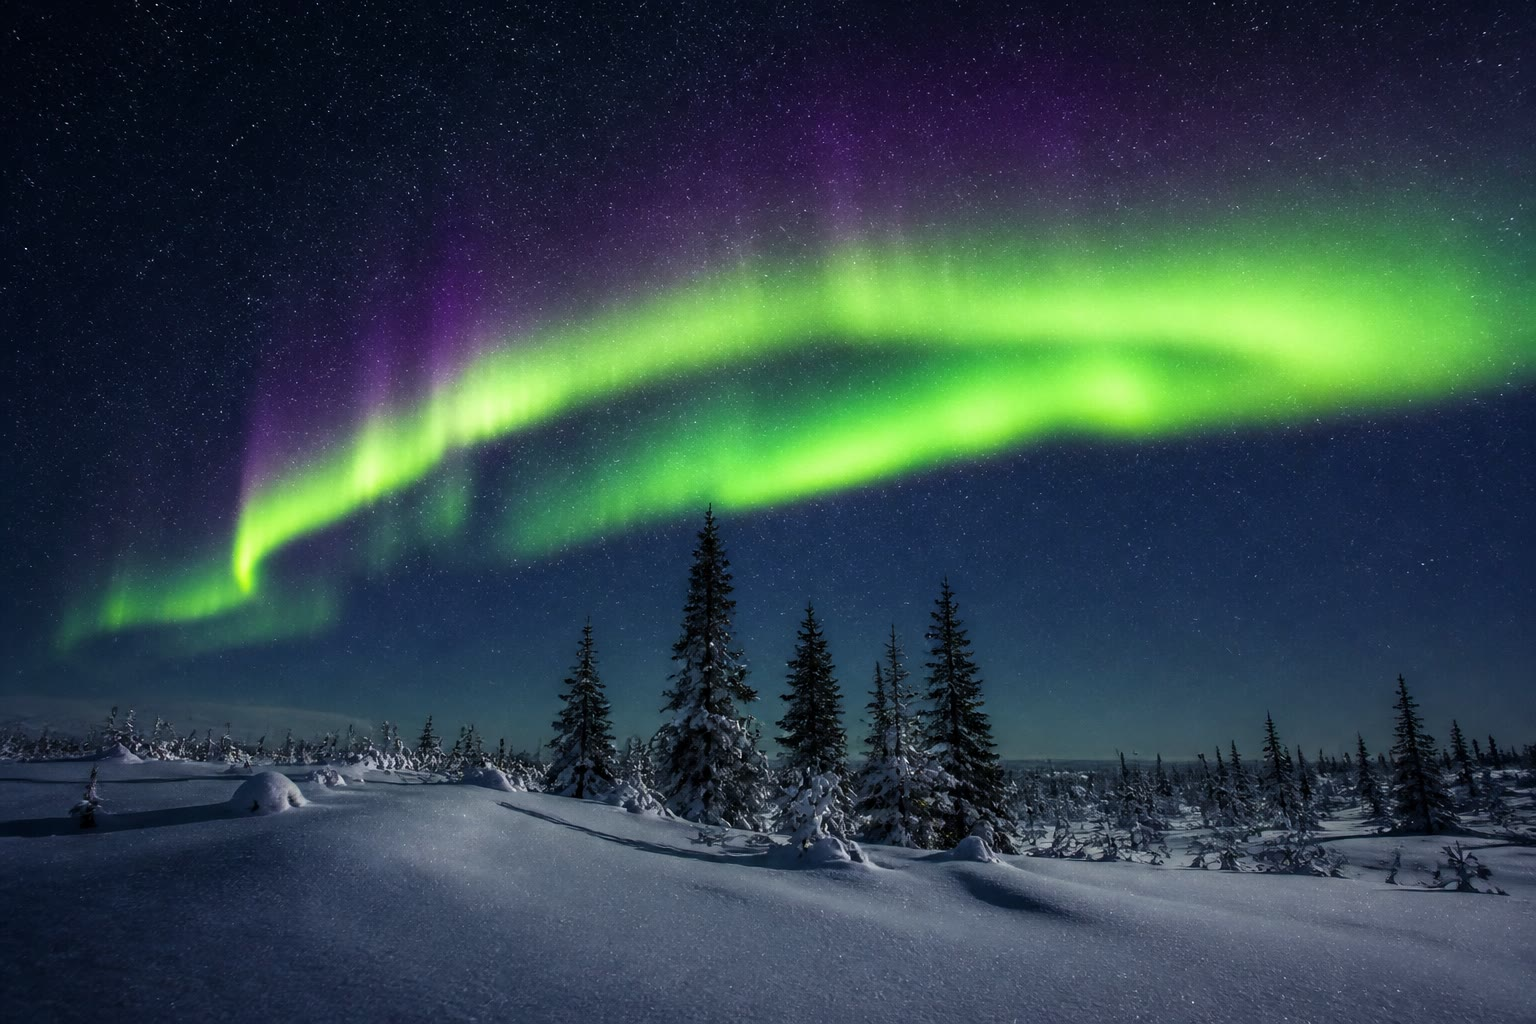
\includegraphics[width=0.58\linewidth]{images/book5/ai/b5-24-aurora-arc.jpg}

{\small 一幅极光：太阳风带电粒子在地磁场的导引下进入极地大气层。一位观测者称之为磁导引，另一位则称之为电加速——各场在本章的变换下相互混合。}
\end{omfigure}

\section{练习}

\begin{exercise}[$\star$]\label{exo:b3:covariant-electromagnetism:1}
(a) 对 $a^\mu = (5, 3, 0, 0)$（以某个 $a_0$ 为单位）作 $\beta =
0.6$ 的洛伦兹变换：求 $a'^\mu$，并验证 $a\cdot a$ 不变。(b) 证明
两个四维矢量之和是四维矢量。(c) 某粒子的 $(c,
\vect v)$ 是否为四维矢量？$\gamma(c, \vect v)$ 呢？(d)
为什么仅“电场”本身不属于任何四维矢量？
\end{exercise}

\begin{exercise}[$\star$]\label{exo:b3:covariant-electromagnetism:2}
一根截面积为 \qty{1.0}{mm^2} 的铜线，通有 \qty{10}{A} 的电流；
传导电子数密度 $n = \qty{8.5e28}{m^{-3}}$。(a) 计算
漂移速率。(b) 写出电子流体与晶格的 $J^\mu$。
(c) 对二者分别检验连续性方程。(d) 导线呈电中性，
因此整根导线的 $J^\mu$ 是多少，
哪一个分量保留下来？
\end{exercise}

\begin{exercise}[$\star$]\label{exo:b3:covariant-electromagnetism:3}
(a) 由 $F^{\mu\nu}$ 的矩阵，读出给出
$E_y$ 与 $B_x$ 的分量。(b) 写出 $F^{\mu\nu}$，分别对应纯均匀场
$\vect B = B\vect e_z$ 与平面波场
（$\vect E = E\vect e_y$，$\vect B = (E/c)\vect e_z$）。(c) 验证
在分量上 $F^{\mu\nu} = \partial^\mu A^\nu - \partial^\nu
A^\mu$ 重现 $\vect B = \operatorname{\vect{curl}}\vect A$，
取 $\mu\nu = 12$。(d) 为什么 $F$ 必须反对称，
才使力 $qF^{\mu\nu}u_\nu$ 在粒子自身参考系中不做功？
\end{exercise}

\begin{exercise}[$\star$]\label{exo:b3:covariant-electromagnetism:4}
一平行板电容器静止，其中 $\vect E = E_0\vect e_y$，
无 $\vect B$。求在运动参考系中的 $\vect E'$ 与 $\vect B'$，运动方向分别为 (a)
沿 $\vect e_y$（垂直于极板）；(b) 沿 $\vect
e_x$（平行于极板），并将出现的 $\vect B'$ 解释为
运动面电荷的场；(c) 检验情形 (b) 中的不变量；
(d) 情形 (b) 中极板也收缩，
哪些量（$\sigma$？$E'$？极板间距？）发生改变，
而它们应与什么保持一致？
\end{exercise}

\begin{exercise}[$\star\star$]\label{exo:b3:covariant-electromagnetism:5}
动生电动势的统一。一根导体棒以 $\vect v$ 的速度沿导轨滑动，
穿过均匀磁场 $\vect B$。(a) 在实验室系中，哪一个力驱动棒中的电子，
产生怎样的电动势？(b) 在导体棒参考系中，
哪一个场驱动它们，它来自
\cref{prop:b3:covariant-electromagnetism:transform}的哪一部分？(c) 证明两种电动势
在 $v/c$ 一阶上一致。(d) 本科一年级分册中的法拉第磁通定则
用一个公式同时涵盖了“运动回路”与“变化场”两种情形，
相对论对于这一统一为何必然成立，
说明了什么？
\end{exercise}

\begin{exercise}[$\star\star$]\label{exo:b3:covariant-electromagnetism:6}
(a) 利用\cref{prop:b3:covariant-electromagnetism:transform}，
直接计算验证 $E'^2 - c^2B'^2 = E^2 - c^2B^2$ 在沿 $x$ 方向的洛伦兹变换下成立。
(b) 验证 $\vect E'\cdot\vect B' = \vect
E\cdot\vect B$。(c) 某区域中 $\vect E$ 与 $\vect B$
互相垂直且 $E = 2cB$：求出只存在电场的参考系（方向与速率）。
(d) 为什么没有任何参考系能使平面光波的场
纯为电场或纯为磁场？
\end{exercise}

\begin{exercise}[$\star\star$]\label{exo:b3:covariant-electromagnetism:7}
交叉场。实验室中 $\vect E = E\vect e_y$ 且 $\vect B =
B\vect e_z$，$E < cB$。(a) 证明以
$\vect v_{\text{d}} = (E/B)\,\vect e_x$ 运动的参考系只看到纯磁场。
(b) 描述从该参考系与实验室中观察，静止释放的电荷的运动
（沿 $v_{\text{d}}$ 漂移的摆线）。(c)
本科一年级分册的速度选择器让速率为 $E/B$ 的粒子不偏转地通过：
由(a)在一行内重新推出这一结论。(d) 定性地说，当 $E > cB$
时会发生什么，
为何此时漂移参考系的技巧不可行？
\end{exercise}

\begin{exercise}[$\star\star$]\label{exo:b3:covariant-electromagnetism:8}
四维波矢 $k^\mu = (\omega/c, \vect k)$。(a) 证明
要求相位不变会迫使 $k^\mu$ 按四维矢量变换。(b) 由其时间分量
推导纵向多普勒公式。(c) 推导光行差公式。(d) 星光
光行差：地球以 \qty{29.8}{km/s} 绕日公转，经一年，
一颗恒星的视位置扫过多大角度？（布拉德利
于 1728 年测得
$20.5''$——这是地球运动的第一个直接证明。）
\end{exercise}

\begin{exercise}[$\star\star$]\label{exo:b3:covariant-electromagnetism:9}
一电荷 $q$ 以恒定速度 $\vect v = v\vect e_x$ 运动，$\gamma \gg
1$。(a) 对库仑场作变换，证明在过电荷的横截面内，
场被增强为 $\gamma
q/4\pi\varepsilon_0b^2$（距离 $b$ 处），而其正前方与正后方
的场被压低为 $1/\gamma^2$ 倍。(b) 证明
距离 $b$ 处的静止观测者会看到时长为
$\sim b/\gamma v$ 的场脉冲。(c) 对于在 $b = \qty{1}{cm}$ 处通过的 LHC 质子：
峰值场与脉冲时长。(d) 这一脉冲在何种确切意义上
“几乎是光”？（检验 $E' \approx cB'$ 及不变量。）
\end{exercise}

\begin{exercise}[$\star\star\star$]\label{exo:b3:covariant-electromagnetism:10}
追逐光波。平面波具有 $\vect E = E_0\vect e_y
\cos(\omega(t - x/c))$，$\vect B = (E_0/c)\vect e_z\cos(\omega(t -
x/c))$。一观测者以 $\beta$ 追赶它。(a) 变换场：
证明 $E'_0 = E_0\sqrt{(1-\beta)/(1+\beta)}$，且 $B'_0 = E'_0/c$。(b)
证明频率以同一因子变换：波仍是波，
发生红移，且始终有 $E' = cB'$。(c) 波的能量密度
（正比于 $E^2$）及光子数如何变化？(d) 归纳：“与光束并肩同行”
需要什么，
哪一个不变量禁止这一点？
\end{exercise}

\begin{exercise}[$\star\star\star$]\label{exo:b3:covariant-electromagnetism:11}
同步辐射与圆形电子加速器的消亡。一个
超相对论电荷在半径为 $r$ 的圆周上辐射功率
$P = q^2c\gamma^4/6\pi\varepsilon_0r^2$（在本阶段不加证明地承认——本科二年级分册的拉莫尔
公式，经相对论推广）。(a) 证明每圈损失的能量
为 $\Delta E = q^2\gamma^4/3\varepsilon_0r$。(b) LEP：电子
能量为 \qty{100}{GeV}，环形轨道 $r = \qty{3.1}{km}$：求 $\gamma$ 及
每圈的 $\Delta E$ ——束流能量中需要每圈补回的比例
是多少？(c) LHC：质子能量为 \qty{6.8}{TeV}，隧道相同：求
每圈的 $\Delta E$，并作比较。(d) 结合因子 $\gamma^4 =
(E/mc^2)^4$，解释为何电子的后继装置是
\emph{直线型}对撞机，或更大的环形装置，以及为何质子环
仍然得以保留。
\end{exercise}

\begin{exercise}[$\star\star\star$]\label{exo:b3:covariant-electromagnetism:12}
相对论回旋加速器。一个电荷处于均匀磁场 $\vect B$ 中，以
相对论速率运动。(a) 由 $\dd\vect p/\dd t = q\vect v\wedge\vect
B$，取 $E$ 不变，证明轨道为圆周，且以
$\omega = qB/\gamma m$ 运行，即回旋频率随能量增大而减小。
(b) 经典回旋加速器以固定的 $\omega_0 = qB/m$ 施加驱动：证明
经过 $N$ 圈后，$\gamma - 1$ 线性增长至终值
$\Gamma$，累积相位滑移达到四分之一射频周期
时，即 $\Gamma \approx 1/2N$；对于 $N = 100$ 圈，质子动能为
多少，它与经典回旋加速器的历史
上限（约 \qty{20}{MeV}
，靠额外的裕量与电压获得）相比如何？(c) 两种补救办法
存在：调频（同步回旋加速器），或将 $B(r)$ 设计为
随 $\gamma$ 增长（等时性回旋加速器）：请各用一句话
说明。(d) PSI 等时性回旋加速器输出 \qty{590}{MeV} 的质子，
其边缘处磁场超过中心磁场的
倍数为多少？
\end{exercise}

\section{问题：蜗速下的磁学}

\begin{problem}[{周末问题——一个 $10^{-24}$ 的失衡如何驱动
每台电动机}]\label{pb:b3:covariant-electromagnetism:1}
电子在灯线中的漂移比蜂蜜的流淌还要慢，
而该漂移的 $v^2/c^2$ 仅为 $10^{-24}$ ——但其产生的磁力
却能在废品场吊起汽车。本题将完整地
对直导线与运动电荷做双参考系的分析，并
揭示每一块电磁铁中隐藏的相对论效应。数据：铜导线，
截面积 $S = \qty{1.0}{mm^2}$，电流 $I = \qty{10}{A}$，
传导电子密度 $n = \qty{8.5e28}{m^{-3}}$；试探电荷
$q = \qty{1}{\micro C}$，位于距导线 $d = \qty{1.0}{cm}$ 处，
平行于导线以 $v = \qty{e5}{m/s}$ 运动（离子束速率，为
使数值清晰可见）；$\mu_0 = 4\pi\times10^{-7}\,\unit{H/m}$。

\medskip\noindent\textbf{第一部分——实验室系中的分析。}
\begin{enumerate}
  \item 计算电子的漂移速率 $u$，以及 $u^2/c^2$。
  \item 将导线建模为两个叠加的线电荷：晶格
        $+\lambda$ 静止，电子 $-\lambda$ 以
        $u$ 漂移，$I = \lambda u$。求 $\lambda$。
  \item 计算电荷位置处的 $B$，以及其所受磁力
        $F = qvB$ ——包括方向，取 $v$ 与
        常规电流 $I$ 平行（回忆：平行电流
        相互吸引）。
  \item 为何实验室系中没有\emph{电场力}？
  \item 设同一导线的净电荷仅为
        每米多出一个电子，比较其对 $q$ 施加的力
        与第 3 题中的磁力，并由此得出
        须将“中性”测到何种精度，
        才能将力归因于磁效应。
  \item 一个 \qty{1}{\micro C} 的电荷、速率为 \qty{e5}{m/s} 时，第 3 题中的力
        是否可测？（与一粒沙子的
        重量 $\sim\qty{e-6}{N}$ 相比）。
\end{enumerate}

\medskip\noindent\textbf{第二部分——换参考系。}
变换到试探电荷的参考系（沿导线方向的速率为 $v$）。
\begin{enumerate}[resume]
  \item 在该参考系中，晶格与
        电子的速度（电子漂移方向与 $I$ 相反，因此在此变换中速率增加
        ——须正确进行速度合成）？
  \item 对导线截面积分后，单位长度的四维电流
        为 $(c\lambda_{\text{总}}, I, 0, 0)$，其中
        $\lambda_{\text{总}} = 0$。对其作变换，证明
        导线在新参考系中的线电荷为
        \[
        \lambda' = -\gamma_v\,\frac{vI}{c^2} .
        \]
  \item 计算 $\lambda'$，分别以库仑每米和每米的电子电荷数表示
        哪一股电荷流变得更密，为什么
        （若愿意，可分别对每股作长度收缩）？
  \item 计算电荷处的电场 $E' = \lambda'/2\pi\varepsilon_0d$，
        以及其所受的电场力 $qE'$。
  \item 将 $qE'$ 与第一部分中实验室系的 $qvB$ 作比较，并解释
        剩余因子 $\gamma_v \approx 1 + \num{5.6e-8}$
        （哪一个四维矢量的变换律联系这两个力？）。
  \item 在该参考系中仍存在磁场（导线
        仍携带电流）：为何它在此处不施力？
\end{enumerate}

\medskip\noindent\textbf{第三部分——数字背后的道理。}
\begin{enumerate}[resume]
  \item 计算相对失衡 $|\lambda'|/\lambda$，
        并写成 $\gamma_v vu/c^2$。
  \item 仅为导线电荷量 $10^{-19}$ 量级的效应，如何
        产生宏观的力？（它所乘的是一个
        多么巨大的数？）
  \item 两根平行导线，各载 \qty{10}{A} 电流，相距 \qty{1}{cm}：
        求单位长度所受的力，并与
        定义精度的值 $2 \times 10^{-7}\,I_1I_2/d$ 牛顿
        每米进行核对。
  \item 电磁铁相当于此故事的一万次重复：
        估算一个 \qty{e4}{}-匝线圈每米的磁场
        通以 \qty{10}{A} 电流（本科一年级分册中的螺线管公式），
        以及其作用于铁上的、每平方厘米的力
        （$\sim B^2/2\mu_0$）。
  \item 若关闭相对论（变换中令 $c \to \infty$），
        则 $\lambda'$ 与 $B$ 的作用力还剩下什么，
        以及电动机与废品场中的磁铁？
  \item 为何导线附近处于\emph{静止}的试探电荷
        感受不到任何作用，尽管电子从旁边流过？（哪一种
        抵消保护了它，且精确到何种程度？）
\end{enumerate}

\medskip\noindent\textbf{第四部分——导线之外。}
\begin{enumerate}[resume]
  \item 第二年分册把电流当作给定源，依据安培环路定理推导磁场。
        本章对这一叙述有何补充——
        从本题来看，磁场\emph{究竟}
        是什么？
  \item 铁质磁铁没有电池：在永磁现象中，
        什么扮演了电流的角色
        （一句话即可；诚实的微观回答是量子性的，留待五章之后再讲）？
  \item 真空中一束单独的电子束（无晶格）：同向运动的观察者
        会认为它比实验室观察者更倾向于吸引还是排斥它自身？
        请调和两个参考系
        对电子束自箍缩的描述。
  \item 将上一点定量化：证明两束平行的同号电荷束，
        以 $\beta$ 同向运动时相互排斥，其
        合力（电排斥减去磁吸引）
        比静止时的值恰好减小 $1/\gamma^2$——并
        说明哪一个参考系的描述使该因子一目了然。
  \item 灯泡的能量以接近 $c$ 的速度到达，
        而其中的电子每小时仅漂移一米：
        究竟是什么沿导线输送能量（回顾
        第二年分册中的坡印廷矢量）？
  \item 估算本题电子以及一个行人式试探电荷的 $vu/c^2$，
        （$v = \qty{1}{m/s}$）：即便在那里，
        力仍可用指南针指针一阶地测得——
        是谁演示了电流使指南针偏转，
        又是哪一年？
  \item 概括这一著名结论：一根中性的、电流为 \qty{10}{A} 的导线，
        从以 \qty{e5}{m/s} 运动的座位上观察，
        带有 $-\qty{e-11}{C/m}$ 的相对论电荷——
        而长度收缩那个数量级为 $10^{-24}$ 的记账误差，
        乘以 $10^{28}$ 个电子，
        便是整个实验室里的全部磁力。
\end{enumerate}
\end{problem}
